% SOURCE: edit-harness/results/frame_a/cells/cell_*_real_MIX_{A,B,C}_*.json
% !TEX encoding = UTF-8 Unicode
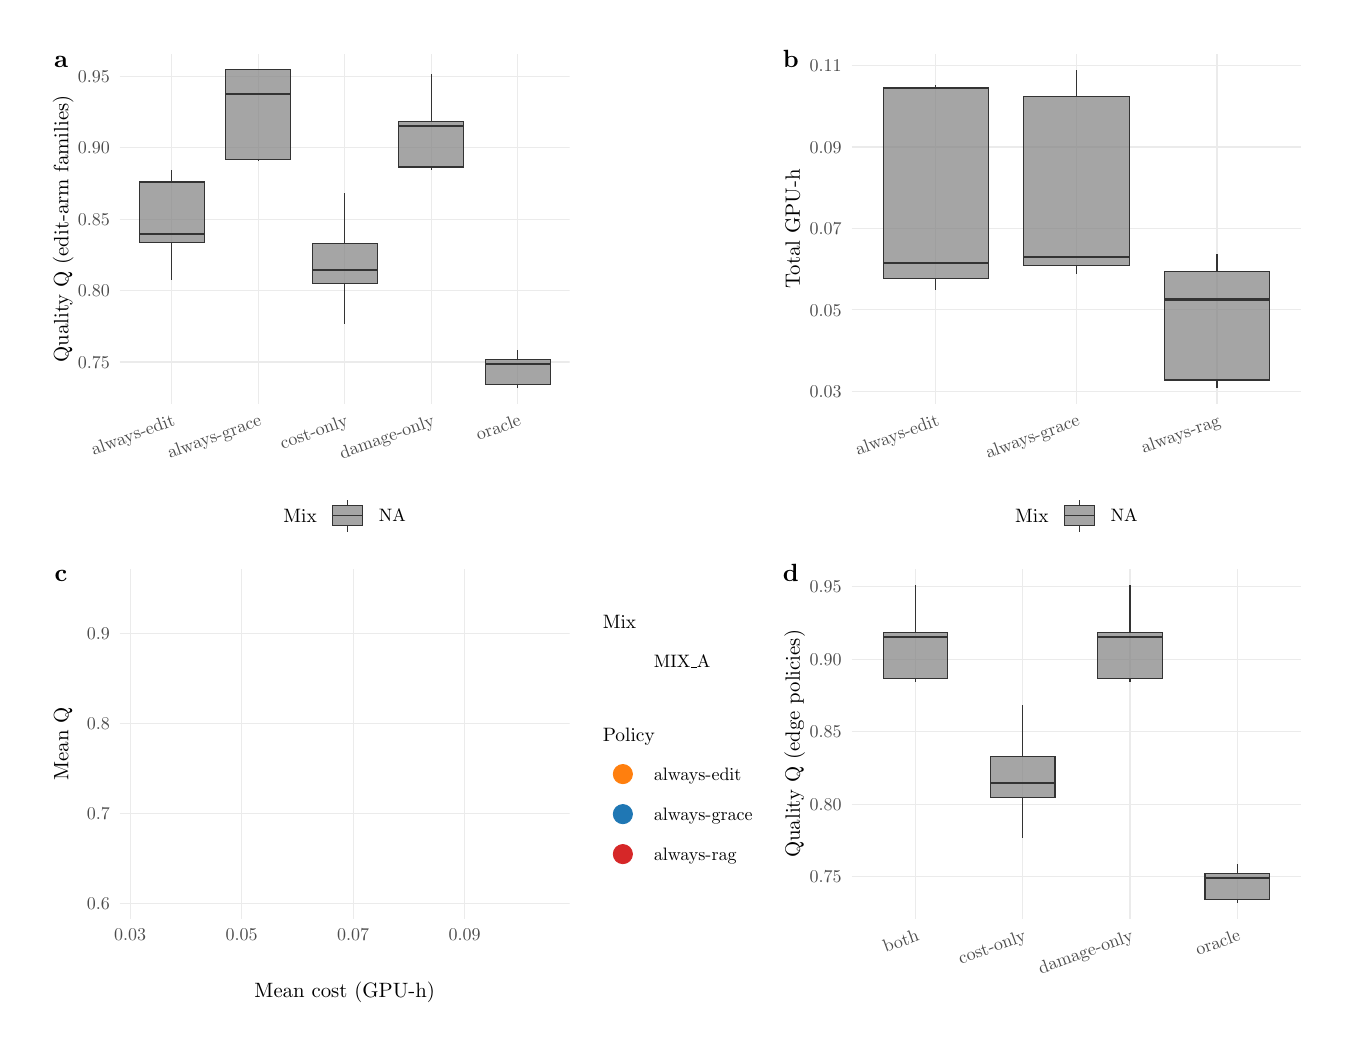
\begin{tikzpicture}[x=1pt,y=1pt]
\definecolor{fillColor}{RGB}{255,255,255}
\path[use as bounding box,fill=fillColor,fill opacity=0.00] (0,0) rectangle (469.75,361.35);
\begin{scope}
\path[clip] (  0.00,  0.00) rectangle (469.75,361.35);
\definecolor{drawColor}{RGB}{255,255,255}
\definecolor{fillColor}{RGB}{255,255,255}

\path[draw=drawColor,line width= 0.6pt,line join=round,line cap=round,fill=fillColor] (  0.00,  0.00) rectangle (469.75,361.35);
\end{scope}
\begin{scope}
\path[clip] (  5.50,169.76) rectangle (269.91,355.85);
\definecolor{fillColor}{RGB}{255,255,255}

\path[fill=fillColor] (  5.50,169.76) rectangle (269.91,355.85);
\end{scope}
\begin{scope}
\path[clip] (269.91,169.76) rectangle (464.25,355.85);
\definecolor{fillColor}{RGB}{255,255,255}

\path[fill=fillColor] (269.91,169.76) rectangle (464.25,355.85);
\end{scope}
\begin{scope}
\path[clip] (  5.50,  5.50) rectangle (269.91,169.76);
\definecolor{fillColor}{RGB}{255,255,255}

\path[fill=fillColor] (  5.50,  5.50) rectangle (269.91,169.76);
\end{scope}
\begin{scope}
\path[clip] (269.91,  5.50) rectangle (464.25,169.76);
\definecolor{fillColor}{RGB}{255,255,255}

\path[fill=fillColor] (269.91,  5.50) rectangle (464.25,169.76);
\end{scope}
\begin{scope}
\path[clip] ( 33.28,225.49) rectangle (195.84,351.85);
\definecolor{drawColor}{gray}{0.92}

\path[draw=drawColor,line width= 0.4pt,line join=round] ( 33.28,240.54) --
	(195.84,240.54);

\path[draw=drawColor,line width= 0.4pt,line join=round] ( 33.28,266.36) --
	(195.84,266.36);

\path[draw=drawColor,line width= 0.4pt,line join=round] ( 33.28,292.19) --
	(195.84,292.19);

\path[draw=drawColor,line width= 0.4pt,line join=round] ( 33.28,318.01) --
	(195.84,318.01);

\path[draw=drawColor,line width= 0.4pt,line join=round] ( 33.28,343.83) --
	(195.84,343.83);

\path[draw=drawColor,line width= 0.4pt,line join=round] ( 52.03,225.49) --
	( 52.03,351.85);

\path[draw=drawColor,line width= 0.4pt,line join=round] ( 83.30,225.49) --
	( 83.30,351.85);

\path[draw=drawColor,line width= 0.4pt,line join=round] (114.56,225.49) --
	(114.56,351.85);

\path[draw=drawColor,line width= 0.4pt,line join=round] (145.82,225.49) --
	(145.82,351.85);

\path[draw=drawColor,line width= 0.4pt,line join=round] (177.09,225.49) --
	(177.09,351.85);
\definecolor{drawColor}{gray}{0.20}

\path[draw=drawColor,line width= 0.4pt,line join=round] ( 52.03,305.57) -- ( 52.03,310.08);

\path[draw=drawColor,line width= 0.4pt,line join=round] ( 52.03,283.61) -- ( 52.03,270.11);
\definecolor{fillColor}{RGB}{127,127,127}

\path[draw=drawColor,line width= 0.4pt,fill=fillColor,fill opacity=0.70] ( 40.31,305.57) --
	( 40.31,283.61) --
	( 63.76,283.61) --
	( 63.76,305.57) --
	( 40.31,305.57) --
	cycle;

\path[draw=drawColor,line width= 0.8pt] ( 40.31,286.73) -- ( 63.76,286.73);

\path[draw=drawColor,line width= 0.4pt,line join=round] ( 83.30,346.11) -- ( 83.30,346.11);

\path[draw=drawColor,line width= 0.4pt,line join=round] ( 83.30,313.87) -- ( 83.30,313.05);

\path[draw=drawColor,line width= 0.4pt,fill=fillColor,fill opacity=0.70] ( 71.57,346.11) --
	( 71.57,313.87) --
	( 95.02,313.87) --
	( 95.02,346.11) --
	( 71.57,346.11) --
	cycle;

\path[draw=drawColor,line width= 0.8pt] ( 71.57,337.43) -- ( 95.02,337.43);

\path[draw=drawColor,line width= 0.4pt,line join=round] (114.56,283.25) -- (114.56,301.65);

\path[draw=drawColor,line width= 0.4pt,line join=round] (114.56,268.80) -- (114.56,254.40);

\path[draw=drawColor,line width= 0.4pt,fill=fillColor,fill opacity=0.70] (102.84,283.25) --
	(102.84,268.80) --
	(126.28,268.80) --
	(126.28,283.25) --
	(102.84,283.25) --
	cycle;

\path[draw=drawColor,line width= 0.8pt] (102.84,273.90) -- (126.28,273.90);

\path[draw=drawColor,line width= 0.4pt,line join=round] (145.82,327.59) -- (145.82,344.51);

\path[draw=drawColor,line width= 0.4pt,line join=round] (145.82,310.99) -- (145.82,309.97);

\path[draw=drawColor,line width= 0.4pt,fill=fillColor,fill opacity=0.70] (134.10,327.59) --
	(134.10,310.99) --
	(157.55,310.99) --
	(157.55,327.59) --
	(134.10,327.59) --
	cycle;

\path[draw=drawColor,line width= 0.8pt] (134.10,325.93) -- (157.55,325.93);

\path[draw=drawColor,line width= 0.4pt,line join=round] (177.09,241.57) -- (177.09,244.88);

\path[draw=drawColor,line width= 0.4pt,line join=round] (177.09,232.48) -- (177.09,231.24);

\path[draw=drawColor,line width= 0.4pt,fill=fillColor,fill opacity=0.70] (165.36,241.57) --
	(165.36,232.48) --
	(188.81,232.48) --
	(188.81,241.57) --
	(165.36,241.57) --
	cycle;

\path[draw=drawColor,line width= 0.8pt] (165.36,239.92) -- (188.81,239.92);
\end{scope}
\begin{scope}
\path[clip] (  0.00,  0.00) rectangle (469.75,361.35);
\definecolor{drawColor}{gray}{0.30}

\node[text=drawColor,anchor=base east,inner sep=0pt, outer sep=0pt, scale=  0.65] at ( 29.68,238.30) {0.75};

\node[text=drawColor,anchor=base east,inner sep=0pt, outer sep=0pt, scale=  0.65] at ( 29.68,264.13) {0.80};

\node[text=drawColor,anchor=base east,inner sep=0pt, outer sep=0pt, scale=  0.65] at ( 29.68,289.95) {0.85};

\node[text=drawColor,anchor=base east,inner sep=0pt, outer sep=0pt, scale=  0.65] at ( 29.68,315.77) {0.90};

\node[text=drawColor,anchor=base east,inner sep=0pt, outer sep=0pt, scale=  0.65] at ( 29.68,341.60) {0.95};
\end{scope}
\begin{scope}
\path[clip] (  0.00,  0.00) rectangle (469.75,361.35);
\definecolor{drawColor}{gray}{0.30}

\node[text=drawColor,rotate= 20.00,anchor=base east,inner sep=0pt, outer sep=0pt, scale=  0.65] at ( 53.56,217.69) {always-edit};

\node[text=drawColor,rotate= 20.00,anchor=base east,inner sep=0pt, outer sep=0pt, scale=  0.65] at ( 84.83,217.69) {always-grace};

\node[text=drawColor,rotate= 20.00,anchor=base east,inner sep=0pt, outer sep=0pt, scale=  0.65] at (116.09,217.69) {cost-only};

\node[text=drawColor,rotate= 20.00,anchor=base east,inner sep=0pt, outer sep=0pt, scale=  0.65] at (147.35,217.69) {damage-only};

\node[text=drawColor,rotate= 20.00,anchor=base east,inner sep=0pt, outer sep=0pt, scale=  0.65] at (178.62,217.69) {oracle};
\end{scope}
\begin{scope}
\path[clip] (  0.00,  0.00) rectangle (469.75,361.35);
\definecolor{drawColor}{RGB}{0,0,0}

\node[text=drawColor,rotate= 90.00,anchor=base,inner sep=0pt, outer sep=0pt, scale=  0.75] at ( 14.67,288.67) {Quality Q (edit-arm families)};
\end{scope}
\begin{scope}
\path[clip] (  0.00,  0.00) rectangle (469.75,361.35);
\definecolor{drawColor}{RGB}{0,0,0}

\node[text=drawColor,anchor=base west,inner sep=0pt, outer sep=0pt, scale=  0.70] at ( 92.43,182.58) {Mix};
\end{scope}
\begin{scope}
\path[clip] (  0.00,  0.00) rectangle (469.75,361.35);
\definecolor{drawColor}{gray}{0.20}

\path[draw=drawColor,line width= 0.4pt] (115.71,179.21) --
	(115.71,181.37);

\path[draw=drawColor,line width= 0.4pt] (115.71,188.60) --
	(115.71,190.77);
\definecolor{fillColor}{RGB}{127,127,127}

\path[draw=drawColor,line width= 0.4pt,fill=fillColor,fill opacity=0.70] (110.29,181.37) rectangle (121.13,188.60);

\path[draw=drawColor,line width= 0.4pt] (110.29,184.99) --
	(121.13,184.99);

\path[draw=drawColor,line width= 0.4pt] (115.71,179.21) --
	(115.71,179.21);

\path[draw=drawColor,line width= 0.4pt] (115.71,190.77) --
	(115.71,190.77);
\end{scope}
\begin{scope}
\path[clip] (  0.00,  0.00) rectangle (469.75,361.35);
\definecolor{drawColor}{RGB}{0,0,0}

\node[text=drawColor,anchor=base west,inner sep=0pt, outer sep=0pt, scale=  0.65] at (126.94,182.75) {NA};
\end{scope}
\begin{scope}
\path[clip] (  0.00,  0.00) rectangle (469.75,361.35);
\definecolor{drawColor}{RGB}{0,0,0}

\node[text=drawColor,anchor=base,inner sep=0pt, outer sep=0pt, scale=  0.90] at ( 12.06,346.96) {\bfseries a};
\end{scope}
\begin{scope}
\path[clip] (297.69,225.49) rectangle (460.25,351.85);
\definecolor{drawColor}{gray}{0.92}

\path[draw=drawColor,line width= 0.4pt,line join=round] (297.69,229.93) --
	(460.25,229.93);

\path[draw=drawColor,line width= 0.4pt,line join=round] (297.69,259.35) --
	(460.25,259.35);

\path[draw=drawColor,line width= 0.4pt,line join=round] (297.69,288.78) --
	(460.25,288.78);

\path[draw=drawColor,line width= 0.4pt,line join=round] (297.69,318.21) --
	(460.25,318.21);

\path[draw=drawColor,line width= 0.4pt,line join=round] (297.69,347.63) --
	(460.25,347.63);

\path[draw=drawColor,line width= 0.4pt,line join=round] (328.17,225.49) --
	(328.17,351.85);

\path[draw=drawColor,line width= 0.4pt,line join=round] (378.97,225.49) --
	(378.97,351.85);

\path[draw=drawColor,line width= 0.4pt,line join=round] (429.77,225.49) --
	(429.77,351.85);
\definecolor{drawColor}{gray}{0.20}

\path[draw=drawColor,line width= 0.4pt,line join=round] (328.17,339.55) -- (328.17,340.77);

\path[draw=drawColor,line width= 0.4pt,line join=round] (328.17,270.79) -- (328.17,266.57);
\definecolor{fillColor}{RGB}{127,127,127}

\path[draw=drawColor,line width= 0.4pt,fill=fillColor,fill opacity=0.70] (309.12,339.55) --
	(309.12,270.79) --
	(347.22,270.79) --
	(347.22,339.55) --
	(309.12,339.55) --
	cycle;

\path[draw=drawColor,line width= 0.8pt] (309.12,276.45) -- (347.22,276.45);

\path[draw=drawColor,line width= 0.4pt,line join=round] (378.97,336.47) -- (378.97,346.11);

\path[draw=drawColor,line width= 0.4pt,line join=round] (378.97,275.45) -- (378.97,272.27);

\path[draw=drawColor,line width= 0.4pt,fill=fillColor,fill opacity=0.70] (359.92,336.47) --
	(359.92,275.45) --
	(398.02,275.45) --
	(398.02,336.47) --
	(359.92,336.47) --
	cycle;

\path[draw=drawColor,line width= 0.8pt] (359.92,278.46) -- (398.02,278.46);

\path[draw=drawColor,line width= 0.4pt,line join=round] (429.77,273.22) -- (429.77,279.48);

\path[draw=drawColor,line width= 0.4pt,line join=round] (429.77,234.04) -- (429.77,231.24);

\path[draw=drawColor,line width= 0.4pt,fill=fillColor,fill opacity=0.70] (410.72,273.22) --
	(410.72,234.04) --
	(448.82,234.04) --
	(448.82,273.22) --
	(410.72,273.22) --
	cycle;

\path[draw=drawColor,line width= 0.8pt] (410.72,263.14) -- (448.82,263.14);
\end{scope}
\begin{scope}
\path[clip] (  0.00,  0.00) rectangle (469.75,361.35);
\definecolor{drawColor}{gray}{0.30}

\node[text=drawColor,anchor=base east,inner sep=0pt, outer sep=0pt, scale=  0.65] at (294.09,227.69) {0.03};

\node[text=drawColor,anchor=base east,inner sep=0pt, outer sep=0pt, scale=  0.65] at (294.09,257.12) {0.05};

\node[text=drawColor,anchor=base east,inner sep=0pt, outer sep=0pt, scale=  0.65] at (294.09,286.54) {0.07};

\node[text=drawColor,anchor=base east,inner sep=0pt, outer sep=0pt, scale=  0.65] at (294.09,315.97) {0.09};

\node[text=drawColor,anchor=base east,inner sep=0pt, outer sep=0pt, scale=  0.65] at (294.09,345.40) {0.11};
\end{scope}
\begin{scope}
\path[clip] (  0.00,  0.00) rectangle (469.75,361.35);
\definecolor{drawColor}{gray}{0.30}

\node[text=drawColor,rotate= 20.00,anchor=base east,inner sep=0pt, outer sep=0pt, scale=  0.65] at (329.70,217.69) {always-edit};

\node[text=drawColor,rotate= 20.00,anchor=base east,inner sep=0pt, outer sep=0pt, scale=  0.65] at (380.50,217.69) {always-grace};

\node[text=drawColor,rotate= 20.00,anchor=base east,inner sep=0pt, outer sep=0pt, scale=  0.65] at (431.30,217.69) {always-rag};
\end{scope}
\begin{scope}
\path[clip] (  0.00,  0.00) rectangle (469.75,361.35);
\definecolor{drawColor}{RGB}{0,0,0}

\node[text=drawColor,rotate= 90.00,anchor=base,inner sep=0pt, outer sep=0pt, scale=  0.75] at (279.08,288.67) {Total GPU-h};
\end{scope}
\begin{scope}
\path[clip] (  0.00,  0.00) rectangle (469.75,361.35);
\definecolor{drawColor}{RGB}{0,0,0}

\node[text=drawColor,anchor=base west,inner sep=0pt, outer sep=0pt, scale=  0.70] at (356.84,182.58) {Mix};
\end{scope}
\begin{scope}
\path[clip] (  0.00,  0.00) rectangle (469.75,361.35);
\definecolor{drawColor}{gray}{0.20}

\path[draw=drawColor,line width= 0.4pt] (380.12,179.21) --
	(380.12,181.37);

\path[draw=drawColor,line width= 0.4pt] (380.12,188.60) --
	(380.12,190.77);
\definecolor{fillColor}{RGB}{127,127,127}

\path[draw=drawColor,line width= 0.4pt,fill=fillColor,fill opacity=0.70] (374.70,181.37) rectangle (385.54,188.60);

\path[draw=drawColor,line width= 0.4pt] (374.70,184.99) --
	(385.54,184.99);

\path[draw=drawColor,line width= 0.4pt] (380.12,179.21) --
	(380.12,179.21);

\path[draw=drawColor,line width= 0.4pt] (380.12,190.77) --
	(380.12,190.77);
\end{scope}
\begin{scope}
\path[clip] (  0.00,  0.00) rectangle (469.75,361.35);
\definecolor{drawColor}{RGB}{0,0,0}

\node[text=drawColor,anchor=base west,inner sep=0pt, outer sep=0pt, scale=  0.65] at (391.35,182.75) {NA};
\end{scope}
\begin{scope}
\path[clip] (  0.00,  0.00) rectangle (469.75,361.35);
\definecolor{drawColor}{RGB}{0,0,0}

\node[text=drawColor,anchor=base,inner sep=0pt, outer sep=0pt, scale=  0.90] at (275.78,346.96) {\bfseries b};
\end{scope}
\begin{scope}
\path[clip] ( 33.28, 39.40) rectangle (195.84,165.76);
\definecolor{drawColor}{gray}{0.92}

\path[draw=drawColor,line width= 0.4pt,line join=round] ( 33.28, 44.89) --
	(195.84, 44.89);

\path[draw=drawColor,line width= 0.4pt,line join=round] ( 33.28, 77.37) --
	(195.84, 77.37);

\path[draw=drawColor,line width= 0.4pt,line join=round] ( 33.28,109.86) --
	(195.84,109.86);

\path[draw=drawColor,line width= 0.4pt,line join=round] ( 33.28,142.34) --
	(195.84,142.34);

\path[draw=drawColor,line width= 0.4pt,line join=round] ( 37.05, 39.40) --
	( 37.05,165.76);

\path[draw=drawColor,line width= 0.4pt,line join=round] ( 77.34, 39.40) --
	( 77.34,165.76);

\path[draw=drawColor,line width= 0.4pt,line join=round] (117.62, 39.40) --
	(117.62,165.76);

\path[draw=drawColor,line width= 0.4pt,line join=round] (157.90, 39.40) --
	(157.90,165.76);
\end{scope}
\begin{scope}
\path[clip] (  0.00,  0.00) rectangle (469.75,361.35);
\definecolor{drawColor}{gray}{0.30}

\node[text=drawColor,anchor=base east,inner sep=0pt, outer sep=0pt, scale=  0.65] at ( 29.68, 42.65) {0.6};

\node[text=drawColor,anchor=base east,inner sep=0pt, outer sep=0pt, scale=  0.65] at ( 29.68, 75.13) {0.7};

\node[text=drawColor,anchor=base east,inner sep=0pt, outer sep=0pt, scale=  0.65] at ( 29.68,107.62) {0.8};

\node[text=drawColor,anchor=base east,inner sep=0pt, outer sep=0pt, scale=  0.65] at ( 29.68,140.11) {0.9};
\end{scope}
\begin{scope}
\path[clip] (  0.00,  0.00) rectangle (469.75,361.35);
\definecolor{drawColor}{gray}{0.30}

\node[text=drawColor,anchor=base,inner sep=0pt, outer sep=0pt, scale=  0.65] at ( 37.05, 31.33) {0.03};

\node[text=drawColor,anchor=base,inner sep=0pt, outer sep=0pt, scale=  0.65] at ( 77.34, 31.33) {0.05};

\node[text=drawColor,anchor=base,inner sep=0pt, outer sep=0pt, scale=  0.65] at (117.62, 31.33) {0.07};

\node[text=drawColor,anchor=base,inner sep=0pt, outer sep=0pt, scale=  0.65] at (157.90, 31.33) {0.09};
\end{scope}
\begin{scope}
\path[clip] (  0.00,  0.00) rectangle (469.75,361.35);
\definecolor{drawColor}{RGB}{0,0,0}

\node[text=drawColor,anchor=base,inner sep=0pt, outer sep=0pt, scale=  0.75] at (114.56, 10.96) {Mean cost (GPU-h)};
\end{scope}
\begin{scope}
\path[clip] (  0.00,  0.00) rectangle (469.75,361.35);
\definecolor{drawColor}{RGB}{0,0,0}

\node[text=drawColor,rotate= 90.00,anchor=base,inner sep=0pt, outer sep=0pt, scale=  0.75] at ( 14.67,102.58) {Mean Q};
\end{scope}
\begin{scope}
\path[clip] (  0.00,  0.00) rectangle (469.75,361.35);
\definecolor{drawColor}{RGB}{0,0,0}

\node[text=drawColor,anchor=base west,inner sep=0pt, outer sep=0pt, scale=  0.70] at (207.84,144.17) {Mix};
\end{scope}
\begin{scope}
\path[clip] (  0.00,  0.00) rectangle (469.75,361.35);
\definecolor{drawColor}{RGB}{0,0,0}

\node[text=drawColor,anchor=base west,inner sep=0pt, outer sep=0pt, scale=  0.65] at (226.30,130.02) {MIX\_A};
\end{scope}
\begin{scope}
\path[clip] (  0.00,  0.00) rectangle (469.75,361.35);
\definecolor{drawColor}{RGB}{0,0,0}

\node[text=drawColor,anchor=base west,inner sep=0pt, outer sep=0pt, scale=  0.70] at (207.84,103.53) {Policy};
\end{scope}
\begin{scope}
\path[clip] (  0.00,  0.00) rectangle (469.75,361.35);
\definecolor{drawColor}{RGB}{255,127,14}
\definecolor{fillColor}{RGB}{255,127,14}

\path[draw=drawColor,line width= 0.3pt,line join=round,line cap=round,fill=fillColor] (215.07, 91.63) circle (  3.47);
\end{scope}
\begin{scope}
\path[clip] (  0.00,  0.00) rectangle (469.75,361.35);
\definecolor{drawColor}{RGB}{31,119,180}
\definecolor{fillColor}{RGB}{31,119,180}

\path[draw=drawColor,line width= 0.3pt,line join=round,line cap=round,fill=fillColor] (215.07, 77.17) circle (  3.47);
\end{scope}
\begin{scope}
\path[clip] (  0.00,  0.00) rectangle (469.75,361.35);
\definecolor{drawColor}{RGB}{214,39,40}
\definecolor{fillColor}{RGB}{214,39,40}

\path[draw=drawColor,line width= 0.3pt,line join=round,line cap=round,fill=fillColor] (215.07, 62.72) circle (  3.47);
\end{scope}
\begin{scope}
\path[clip] (  0.00,  0.00) rectangle (469.75,361.35);
\definecolor{drawColor}{RGB}{0,0,0}

\node[text=drawColor,anchor=base west,inner sep=0pt, outer sep=0pt, scale=  0.65] at (226.30, 89.39) {always-edit};
\end{scope}
\begin{scope}
\path[clip] (  0.00,  0.00) rectangle (469.75,361.35);
\definecolor{drawColor}{RGB}{0,0,0}

\node[text=drawColor,anchor=base west,inner sep=0pt, outer sep=0pt, scale=  0.65] at (226.30, 74.93) {always-grace};
\end{scope}
\begin{scope}
\path[clip] (  0.00,  0.00) rectangle (469.75,361.35);
\definecolor{drawColor}{RGB}{0,0,0}

\node[text=drawColor,anchor=base west,inner sep=0pt, outer sep=0pt, scale=  0.65] at (226.30, 60.48) {always-rag};
\end{scope}
\begin{scope}
\path[clip] (  0.00,  0.00) rectangle (469.75,361.35);
\definecolor{drawColor}{RGB}{0,0,0}

\node[text=drawColor,anchor=base,inner sep=0pt, outer sep=0pt, scale=  0.90] at ( 12.06,161.09) {\bfseries c};
\end{scope}
\begin{scope}
\path[clip] (297.69, 39.40) rectangle (460.25,165.76);
\definecolor{drawColor}{gray}{0.92}

\path[draw=drawColor,line width= 0.4pt,line join=round] (297.69, 54.58) --
	(460.25, 54.58);

\path[draw=drawColor,line width= 0.4pt,line join=round] (297.69, 80.77) --
	(460.25, 80.77);

\path[draw=drawColor,line width= 0.4pt,line join=round] (297.69,106.96) --
	(460.25,106.96);

\path[draw=drawColor,line width= 0.4pt,line join=round] (297.69,133.14) --
	(460.25,133.14);

\path[draw=drawColor,line width= 0.4pt,line join=round] (297.69,159.33) --
	(460.25,159.33);

\path[draw=drawColor,line width= 0.4pt,line join=round] (320.91, 39.40) --
	(320.91,165.76);

\path[draw=drawColor,line width= 0.4pt,line join=round] (359.62, 39.40) --
	(359.62,165.76);

\path[draw=drawColor,line width= 0.4pt,line join=round] (398.32, 39.40) --
	(398.32,165.76);

\path[draw=drawColor,line width= 0.4pt,line join=round] (437.03, 39.40) --
	(437.03,165.76);
\definecolor{drawColor}{gray}{0.20}

\path[draw=drawColor,line width= 0.4pt,line join=round] (320.91,142.86) -- (320.91,160.02);

\path[draw=drawColor,line width= 0.4pt,line join=round] (320.91,126.03) -- (320.91,124.99);
\definecolor{fillColor}{RGB}{127,127,127}

\path[draw=drawColor,line width= 0.4pt,fill=fillColor,fill opacity=0.70] (309.30,142.86) --
	(309.30,126.03) --
	(332.52,126.03) --
	(332.52,142.86) --
	(309.30,142.86) --
	cycle;

\path[draw=drawColor,line width= 0.8pt] (309.30,141.17) -- (332.52,141.17);

\path[draw=drawColor,line width= 0.4pt,line join=round] (359.62, 97.89) -- (359.62,116.56);

\path[draw=drawColor,line width= 0.4pt,line join=round] (359.62, 83.24) -- (359.62, 68.64);

\path[draw=drawColor,line width= 0.4pt,fill=fillColor,fill opacity=0.70] (348.01, 97.89) --
	(348.01, 83.24) --
	(371.23, 83.24) --
	(371.23, 97.89) --
	(348.01, 97.89) --
	cycle;

\path[draw=drawColor,line width= 0.8pt] (348.01, 88.41) -- (371.23, 88.41);

\path[draw=drawColor,line width= 0.4pt,line join=round] (398.32,142.86) -- (398.32,160.02);

\path[draw=drawColor,line width= 0.4pt,line join=round] (398.32,126.03) -- (398.32,124.99);

\path[draw=drawColor,line width= 0.4pt,fill=fillColor,fill opacity=0.70] (386.71,142.86) --
	(386.71,126.03) --
	(409.94,126.03) --
	(409.94,142.86) --
	(386.71,142.86) --
	cycle;

\path[draw=drawColor,line width= 0.8pt] (386.71,141.17) -- (409.94,141.17);

\path[draw=drawColor,line width= 0.4pt,line join=round] (437.03, 55.63) -- (437.03, 58.98);

\path[draw=drawColor,line width= 0.4pt,line join=round] (437.03, 46.41) -- (437.03, 45.15);

\path[draw=drawColor,line width= 0.4pt,fill=fillColor,fill opacity=0.70] (425.42, 55.63) --
	(425.42, 46.41) --
	(448.64, 46.41) --
	(448.64, 55.63) --
	(425.42, 55.63) --
	cycle;

\path[draw=drawColor,line width= 0.8pt] (425.42, 53.95) -- (448.64, 53.95);
\end{scope}
\begin{scope}
\path[clip] (  0.00,  0.00) rectangle (469.75,361.35);
\definecolor{drawColor}{gray}{0.30}

\node[text=drawColor,anchor=base east,inner sep=0pt, outer sep=0pt, scale=  0.65] at (294.09, 52.34) {0.75};

\node[text=drawColor,anchor=base east,inner sep=0pt, outer sep=0pt, scale=  0.65] at (294.09, 78.53) {0.80};

\node[text=drawColor,anchor=base east,inner sep=0pt, outer sep=0pt, scale=  0.65] at (294.09,104.72) {0.85};

\node[text=drawColor,anchor=base east,inner sep=0pt, outer sep=0pt, scale=  0.65] at (294.09,130.90) {0.90};

\node[text=drawColor,anchor=base east,inner sep=0pt, outer sep=0pt, scale=  0.65] at (294.09,157.09) {0.95};
\end{scope}
\begin{scope}
\path[clip] (  0.00,  0.00) rectangle (469.75,361.35);
\definecolor{drawColor}{gray}{0.30}

\node[text=drawColor,rotate= 20.00,anchor=base east,inner sep=0pt, outer sep=0pt, scale=  0.65] at (322.44, 31.60) {both};

\node[text=drawColor,rotate= 20.00,anchor=base east,inner sep=0pt, outer sep=0pt, scale=  0.65] at (361.15, 31.60) {cost-only};

\node[text=drawColor,rotate= 20.00,anchor=base east,inner sep=0pt, outer sep=0pt, scale=  0.65] at (399.86, 31.60) {damage-only};

\node[text=drawColor,rotate= 20.00,anchor=base east,inner sep=0pt, outer sep=0pt, scale=  0.65] at (438.56, 31.60) {oracle};
\end{scope}
\begin{scope}
\path[clip] (  0.00,  0.00) rectangle (469.75,361.35);
\definecolor{drawColor}{RGB}{0,0,0}

\node[text=drawColor,rotate= 90.00,anchor=base,inner sep=0pt, outer sep=0pt, scale=  0.75] at (279.08,102.58) {Quality Q (edge policies)};
\end{scope}
\begin{scope}
\path[clip] (  0.00,  0.00) rectangle (469.75,361.35);
\definecolor{drawColor}{RGB}{0,0,0}

\node[text=drawColor,anchor=base,inner sep=0pt, outer sep=0pt, scale=  0.90] at (275.78,161.09) {\bfseries d};
\end{scope}
\end{tikzpicture}
